\documentclass{amsart}

% Packages
\usepackage{amsmath,amssymb,amsthm}
\usepackage{mathtools}
\usepackage{fancyhdr}
\usepackage{lastpage}
\usepackage{cancel}
\usepackage{graphicx}
\usepackage{float}
\usepackage{blindtext}
\usepackage[backend=biber, style=numeric, sorting=none]{biblatex}
\addbibresource{references.bib}
\usepackage{hyperref}
\usepackage{etoolbox}
\usepackage{tikz}
\usetikzlibrary{patterns, decorations.pathreplacing, arrows.meta, positioning, calc}
\makeatletter
\patchcmd{\@sect}{\@secnumpunct}{\space}{}{}
\makeatother

% Document info
\title{Elliptic Curve Cryptography and Group Theory}
\author{
            Deepak Jassal
            \and
            Cory Stecyk
        }
\date{December 5, 2025}

% Theorem system
\newtheorem{thm}{Theorem}[section]
\newtheorem{cor}[thm]{Corollary}
\newtheorem{prop}[thm]{Proposition}
\newtheorem{lem}[thm]{Lemma}
\newtheorem{conj}[thm]{Conjecture}
\newtheorem{quest}[thm]{Question}
\newtheorem{prob}[thm]{Problem}

\theoremstyle{definition}
\newtheorem{defn}[thm]{Definition}
\newtheorem{defns}[thm]{Definitions}
\newtheorem{con}[thm]{Construction}
\newtheorem{exmp}[thm]{Example}
\newtheorem{exmps}[thm]{Examples}
\newtheorem{notn}[thm]{Notation}
\newtheorem{notns}[thm]{Notations}
\newtheorem{addm}[thm]{Addendum}
\newtheorem{exer}[thm]{Exercise}

\theoremstyle{remark}
\newtheorem{rem}[thm]{Remark}
\newtheorem{rems}[thm]{Remarks}
\newtheorem{warn}[thm]{Warning}
\newtheorem{sch}[thm]{Scholium}



\begin{document}
\newpage
\begin{abstract}
    Elliptic Curve Cryptography (ECC) represents a powerful application of abstract algebra to modern cryptography, offering equivalent security to traditional systems with significantly smaller key sizes. This paper investigates the group-theoretic foundations of ECC, beginning with the definition of elliptic curves over finite fields and their associated group structure. We provide explicit formulas for point addition and doubling, accompanied by geometric interpretations and computational examples. 

    Central to our discussion is the Elliptic Curve Discrete Logarithm Problem (ECDLP), whose computational hardness underpins ECC's security advantages over systems like RSA. We demonstrate these concepts through a complete implementation of the Elliptic Curve Diffie-Hellman key exchange protocol, including detailed numerical computations over $\mathbb{F}_{23}$. By connecting theoretical results from group theory and number theory to practical cryptographic applications, this paper showcases the profound interplay between pure mathematics and real-world security systems.
\end{abstract}
\maketitle

\section{Introduction}
Elliptic Cruve Cryptography (ECC) is powerful tool in modern day public-key cryptography. Where systems like RSA (Rivest-Shamir-Adelman) public-key cryptography needs 4096 bits, ECC needs only about 313 bits for the same level of security \cite{Washington2008}. This gives ECC the advantage of being more efficient, meaning less computational power is needed to implement, making it cheaper. This makes them very useful in resource constrained enviroments such as mobile devices.

\indent ECC is an example of something that was at first studied in a strictly pure math enviroment \cite{Washington2008, LozanoRobledo2011} which was then implemented to a non-pure math setting \cite{Washington2008}. Elliptic curves were first studied as objects in number theory and algebraic geometry. Fermat's Last Theorem was proven By Andrew Wiles in 1994 by proving a special case of the modulatiry theorem for the Frey curve \cite{Washington2008, LozanoRobledo2011}. In the mid to late 1980 Neal Koblitz and Victor Miller independantly using the points of elliptic curves in finite fields as the foundation for a cryptography system \cite{Washington2008, Koblitz1994}. 

\indent This paper is organized to first lay the necessecary groundwork for one to understand elliptic curves in this algebraic context. Next, will be mathematical constraints of RSA add ECC systems moving into the elliptic curve discrete logarithm problem and the Group Law. Finally a worked through example of an elliptic curve Diffie Helman key exchange protocol will be given.

\section{Background}
To understand ECC we must first understand the geometry and algebra behind elliptic curves.
\begin{defn}[Finite Field]\label{ff}
    A finite field $F$ is a field with finite order. A field is a set of numbers on which addition, subtraction, multiplication, and division (by non-zero elements) is well defined. 
\end{defn} 
\begin{defn}[Elliptic Curves over Finite Fields]\label{defn:ECC-FF}
    In the context of cryptography, an elliptic curve $E$ over a finite field $\mathbb{F}_q$ ($q=p^k,\,p\geq3$) is defined by the Weierstrass equation 
    \begin{equation}\label{eqn:EC}
        y^2=x^3+ax+b
    \end{equation}
    where $a,b,x,y\in\mathbb{Z}_q$, and $a,b$ are chosen such that $\Delta=16\left(4a^3+27b^2\right)\neq 0$ in $\mathbb{Z}_q$, this is so that the polynomial (\ref{eqn:EC}) has no repeated roots \cite{Washington2008, LozanoRobledo2011, Koblitz1994, RubinsteinSalzedo2018}.\\ 
    We define the set $E(\mathbb{Z}_q)=\left\{(x,y)\in \mathbb{Z}_q\times\mathbb{Z}_q:y^2\equiv x^3+Ax+B\mod p\right\}\cup \{\mathcal{O}\}$, where $\mathcal{O}$ is a point at infinity. 
\end{defn}
Since we are discussing elliptic curves over a finite field in a group theory context it only makes sense to define a binary operation between two points on the curve.

\begin{exmp}[Elliptic Curve]
    \begin{figure}[h!]
    \centering
\begin{tikzpicture}[scale=1.1]
    % Axes
    \draw[->] (-2.5,0) -- (2.5,0) node[right] {$x$};
    \draw[->] (0,-4) -- (0,4) node[above] {$y$};
    \draw[dashed, gray] (-2.5,0) -- (2.5,0);
    
    % Elliptic curve: y^2 = x^3 - x + 1
    \draw[domain=-1.3247:2,samples=150,smooth,variable=\x,blue,thick] 
        plot ({\x},{sqrt(\x^3 - \x + 1)});
    \draw[domain=-1.3247:2,samples=150,smooth,variable=\x,blue,thick] 
        plot ({\x},{-sqrt(\x^3 - \x + 1)});
    
    % Highlight the x-intercept (where y=0)
    \draw[fill=white] (-1.3247,0) circle (2pt) node[below left] {$x \approx -1.32$};
    
    % Add a sample point
    \node[circle,draw=black,fill=red,inner sep=2pt] (sample) at (0,1) {};
    \node[above right] at (0,1) {$(0,1)$};
    
    \node[blue,right] at (1.5,3) {$y^2 = x^3 - x + 1$};
\end{tikzpicture}
    \caption{The elliptic curve $y^2 = x^3 - x + 1$ over $\mathbb{R}$. 
            The curve consists of two symmetric branches (positive and negative $y$)
            that meet at the x-axis where $y=0$. Over $\mathbb{R}$, these form a 
            continuous curve; over finite fields, we consider only discrete points 
            satisfying the equation.}
    \label{fig:classic_ec}
    \end{figure}
\end{exmp}




\begin{defn}[Point Addition on an Elliptic Curve $E$]\label{dfn:paec}
    Let $E$ be an elliptic curve over a finite field $\mathbb{F}_q$ defined by the equation (\ref{eqn:EC}). We define point addition $\oplus$ for points in $E(\mathbb{F}_q)$ as follows:

    \textbf{Geometric Definition (over $\mathbb{R}$ for intuition):}
    Let $A, B \in E(\mathbb{F}_q)$.
    \begin{itemize}
        \item \textbf{Identity:} The point at infinity $\mathcal{O}$ is the additive identity. Thus, for any point $P$, $P \oplus \mathcal{O} = \mathcal{O} \oplus P = P$.
        \item \textbf{Negative:} The negative of a point $A = (x_1, y_1)$ is its reflection over the x-axis, $-A = (x_1, -y_1)$. By the curve equation, $-A$ is also on the curve. By definition, $A \oplus (-A) = \mathcal{O}$.
        \item \textbf{Addition ($A \neq \mathcal{O}, B \neq \mathcal{O}, A \neq \pm B$):} Draw the line $\overline{AB}$ through $A$ and $B$. This line intersects the curve at a third point $C'$. Then $A \oplus B$ is defined as $-C'$, the reflection of $C'$ over the x-axis.
        \item \textbf{Doubling ($A = B$):} Draw the tangent line to the curve at point $A$. This line intersects the curve at another point $C'$. Then $A \oplus A = 2A$ is defined as $-C'$.
    \end{itemize}

    \textbf{Algebraic Definition (for computation in $\mathbb{F}_q$):}
    Let $A = (x_1, y_1)$ and $B = (x_2, y_2)$ be points on $E(\mathbb{F}_q)$.
    \begin{itemize}
        \item If $A = \mathcal{O}$, then $A \oplus B = B$.
        \item If $B = \mathcal{O}$, then $A \oplus B = A$.
        \item Else, if $x_1 = x_2$ and $y_1 = -y_2$ (i.e., $A = -B$), then $A \oplus B = \mathcal{O}$.
        \item Else, if $A \neq B$ (general addition), let the slope $m$ be:
              \[
              m = \frac{y_2 - y_1}{x_2 - x_1} \mod p
              \]
        \item Else, if $A = B$ (point doubling), let the slope $m$ be:
              \[
              m = \frac{3x_1^2 + a}{2y_1} \mod p
              \]
        \item Then, the coordinates of $A \oplus B = (x_3, y_3)$ are given by:
              \[
              x_3 = m^2 - x_1 - x_2 \mod p, \quad y_3 = m(x_1 - x_3) - y_1 \mod p
              \]
    \end{itemize}
\end{defn}
\begin{exmp}[Point Addition on an Elliptic Curve]\label{ex:point-addition}
    Let \(E\) be the elliptic curve over \(\mathbb{F}_{23}\) given by \(y^{2} = x^{3} + x + 4\). 
    Consider points \(A = (0, 2)\) and \(B = (13, 12)\).

    Using the formulas from Definition~\ref{dfn:paec}, we compute \(A \oplus B\):

    \begin{itemize}
        \item Since \(A \neq B\) and \(A \neq -B\), we use the general addition formula.
        
        \item Compute slope:
        \begin{align*}
            m &= \frac{y_2 - y_1}{x_2 - x_1} = \frac{12 - 2}{13 - 0} = \frac{10}{13} \mod 23 \\
              &= 10 \times 13^{-1} \mod 23 \\
              &= 10 \times 16 \mod 23 \quad (\text{since } 13 \times 16 \equiv 1 \mod 23) \\
              &= 160 \mod 23 = 22.
        \end{align*}

        \item Compute \(x_3\):
        \[
        x_3 = m^{2} - x_1 - x_2 = 22^{2} - 0 - 13 = 484 - 13 = 471 \equiv 11 \ (\text{mod } 23).
        \]

        \item Compute \(y_3\):
        \[
        y_3 = m(x_1 - x_3) - y_1 = 22(0 - 11) - 2 = -242 - 2 = -244 \equiv 4 \ (\text{mod } 23).
        \]
    \end{itemize}

    Therefore, \(A \oplus B = (11, 4)\).

    \noindent\textit{Verification:} We check that \((11, 4)\) satisfies the curve equation:
    \[
    4^{2} = 16 \equiv 11^{3} + 11 + 4 = 1331 + 11 + 4 = 1346 \equiv 16 \ (\text{mod } 23).
    \]
    Thus \((11, 4) \in E(\mathbb{F}_{23})\).
\end{exmp}

\begin{figure}[h!]
\centering
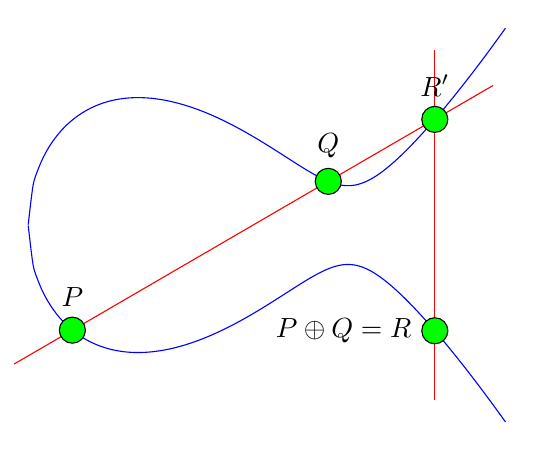
\begin{tikzpicture}[yscale=0.5]
			%TODO: up sample size
			\draw[domain=-4.060646:2,samples=100,smooth,variable=\x,blue] plot ({\x},{sqrt(\x^3 + 4*(\x)^2 + 1)});
			\draw[domain=-4.060646:2,samples=100,smooth,variable=\x,blue] plot ({\x},{-sqrt(\x^3 + 4*(\x)^2 + 1)});
			\node (P) at (-3.5, -2.66926956300783) {};
			\node (Q) at (-0.25, 1.1102430216445) {};
			\node (R) at (1.10295826812394, 2.68474117626385) {};
			\node (P+Q) at (1.10295826812394, -2.68474117626385) {};
			\draw[color=red,shorten >=-1cm,shorten <=-1cm] (P) -- (R);
			\draw[color=red,shorten >=-1cm,shorten <=-1cm] (R) -- (P+Q);
			\node[circle,draw=black,fill=green,label=above:{$P$}] at (P) {};
			\node[circle,draw=black,fill=green,label=above:{$Q$}] at (Q) {};
			\node[circle,draw=black,fill=green,label=above:{$R'$}] at (R) {};
			\node[circle,draw=black,fill=green,label=left:{$P\oplus Q=R$}] at (P+Q) {};
\end{tikzpicture}
\caption{Point addition on an elliptic curve: Given points $P$ and $Q$, 
         draw the line through them (red dashed). This line intersects the curve 
         at a third point $R'$. The sum $P \oplus Q$ is defined as $R$, the 
         reflection of $R'$ over the $x$-axis (green arrow). This geometric 
         construction underlies the algebraic formulas used over finite fields. Credit to \cite{Scholl2019} for this example.}
\label{fig:point_addition}
\end{figure}



\begin{defn}[Diffie-Hellman Key Exchange Protocol]\label{DHKEP}
    The Diffie-Hellman Key Exchange protocol is a method used by two parties, conventionally named Alice and Bob, to agree upon a common secret key which they can then use for exchanging data via a symmetric encryption scheme \cite{Washington2008}. The security of the protocol is based on the difficulty of the Diffie-Hellman Problem (DHP), which is the computational challenge of determining the shared secret given only the public information (Rubenstein-Salzedo)
\end{defn}

\begin{prob}[Discrete Logarithm Problem (DLP)]\label{pb:dlp}
    Given $\alpha\in G$ and $\beta\in\langle\alpha\rangle$, find the least positive integer $x$ such that $x\alpha = \beta$ \cite{Sutherland2015}.
\end{prob}
The DLP is why breaking encrypted messages is so difficult. Trying to find $x$ by brute force is very impractical since the easiest solution to prevent this attack from working is simply picking a very large $x$. It is general consensus that there is not a polynomial time algorithm to find $x$ \cite{Sutherland2015}.
\begin{prob}[Elliptic Curve Discrete Logarithm Problem (ECDLP)]\label{pb:ecdlp}
    Let $E$ be an elliptic curve over a finite field $\mathbb{F}_q$. Let $P\in E(\mathbb{F}_q)$ with $|P|=n$, and let $Q\in\langle P\rangle$. Then $Q=kP=\underbrace{P\oplus P\oplus \cdots\oplus P}_{k\text{ times}}$ for some $k\in\mathbb{F}$. We call $k$ the discrete logarithm of $Q$ with respect to P.
\end{prob}
\section{Main Results}
Perhaps something that may be surprising about the set $E(\mathbb{F}_q)$ with the binary operation $\oplus$ defined in definition (\ref{dfn:paec}) is an Abelian group. With this we move onto our first theorem.
\begin{thm}[]\label{thm:gp-law}
    The group $(E(\mathbb{F}_q),\oplus)$ is an Abelian group.
\end{thm}
\begin{proof}
    Closeure under $\oplus$ is apparent from the fact that by definition the resulting value is another point on the elliptic curve. Commutativity can be easily seen from either the geometric interpretation of definition (\ref{dfn:paec}) or from the formulas. As the lines $\overline{AB}$ and $\overline{BA}$ are the same exacts lines. The identity element in this group is $\mathcal{O}$. If $A=(x_1,y_1)\in E(\mathbb{F}_q)$ then it can be seen from definition (\ref{dfn:paec}) that $A^{-1}=(x_1,-y_1)\in E(\mathbb{F}_q)$, then $A\oplus A^{-1}=\mathcal{O}=e_{E{\mathbb{F}_q}}$.\\
    All that is left to show that $(E(\mathbb{F}_q),\oplus)$ is a group is that associativity holds. This is not at all apparently obvious from either the geometric or algebraic definition given in (\ref{dfn:paec}). In fact, this is quite a complicated proof and it beyond the scope of this paper, so we refer the reader to \textsection 2.4 of \textit{Elliptic Curves Number Theory and Cryptography} by \textit{Lawrence C. Washington}.
\end{proof}
\begin{thm}[Elliptic Curve Security]\label{thm:ecdlp}
    ECC is more secure than RSA, and the security of ECC is realiant on the computational difficultly of the ECDLP.
\end{thm}
\noindent\textit{Explanation.} The reason we present an explanation instead of a proof can be extrapolated from the explanation.\\ 
For RSA there are sub-exponential time algorithms such as the Index Calculus Method \cite{Washington2008} than can be used to solve the discrete log problem. However for the ECDLG (elliptic curve discrete logarithm problem) there are no known sub-exponential time algorithms. Some of the best known algorithms such as Pollard's $\rho$ algorithm have a running time of $O(\sqrt{n})$, where $n$ is the subgroup order \cite{Washington2008}. So far, it has not been shown that a sub-exponential time algorithm exists of the ECDLP. So the fact that a non sub-exponential time algorithm does not exist is not a fact, but rather an assumption. This assumption is similar to how factoring large integers into primes is hard is an assumption for the RSA crytpo system.



\section{Examples and Applications}

\subsection*{Example: Constructing a Small Elliptic Curve Group}

To illustrate the concepts defined above, we will construct a small elliptic curve group and perform point addition.

Let us define an elliptic curve over the finite field $\mathbb{F}_{23}$. We choose $a = 1$ and $b = 4$ for our curve equation $y^2 = x^3 + x + 4$. First, we verify the curve is non-singular (i.e., $\Delta\neq0$) by checking the discriminant $\Delta$:
\[
\Delta = -16(4a^3 + 27b^2) = -16(4(1)^3 + 27(4)^2) = -16(4 + 432) = -6976.
\]
Working modulo $23$, we find $-6976 \equiv 9 \not\equiv 0 \pmod{23}$. Thus, the curve is non-singular.

Our elliptic curve is defined as:
\[
E(\mathbb{F}_{23}): y^2 = x^3 + x + 4.
\]
The set of points $E(\mathbb{F}_{23})$ consists of all pairs $(x, y) \in \mathbb{F}_{23} \times \mathbb{F}_{23}$ satisfying this equation, along with the point at infinity $\mathcal{O}$.

Let us find the point $P = (0, 2)$. Substituting into the curve equation:
\[
2^2 = 4 \equiv 0^3 + 0 + 4 \equiv 4 \pmod{23}.
\]
The equation holds, so $P$ is on the curve. We will now compute $2P = P \oplus P$ using the point doubling formulas from Definition \ref{dfn:paec}.

\begin{itemize}
    \item Since $A = B = (0, 2)$, we use the point doubling formula.
    \item Calculate the slope $m$:
    \[
    m = \frac{3x_1^2 + a}{2y_1} = \frac{3(0)^2 + 1}{2 \cdot 2} = \frac{1}{4} \mod 23.
    \]
    We need the multiplicative inverse of $4$ modulo $23$. Since $4 \times 6 = 24 \equiv 1 \pmod{23}$, the inverse is $6$.
    \[
    m = 1 \times 6 = 6 \mod 23.
    \]
    \item Now calculate $x_3$:
    \[
    x_3 = m^2 - x_1 - x_2 = 6^2 - 0 - 0 = 36 \equiv 13 \pmod{23}.
    \]
    \item Finally, calculate $y_3$:
    \[
    y_3 = m(x_1 - x_3) - y_1 = 6(0 - 13) - 2 = 6(-13) - 2 = -78 - 2 = -80 \pmod{23}.
    \]
    Since $-80 \div 23 = -4$ with a remainder of $12$ ($-80 - (-4\times23) = -80 + 92 = 12$), we have:
    \[
    y_3 \equiv 12 \pmod{23}.
    \]
\end{itemize}

Therefore, $2P = (13, 12)$. The reader can verify that $(13, 12)$ is indeed a point on the curve $E$. By continuing this process, one can compute the entire group. It can be shown that $E(\mathbb{F}_{23})$ has $29$ points ($28$ finite points and $\mathcal{O}$) and is a cyclic group.

\subsection*{Application: Elliptic Curve Diffie-Hellman Key Exchange (ECDH)}

The Elliptic Curve Diffie-Hellman (ECDH) protocol is a direct application of the group law on elliptic curves and the hardness of the ECDLP. It allows two parties, Alice and Bob, to establish a shared secret over an insecure channel.

\subsubsection*{Protocol Setup}

\begin{enumerate}
    \item \textbf{Public Parameters:} Alice and Bob publicly agree on:
    \begin{itemize}
        \item An elliptic curve $E$ defined over a finite field $\mathbb{F}_q$.
        \item A base point $P \in E(\mathbb{F}_q)$ with large prime order $n$. (The subgroup $\langle P \rangle$ is large and cyclic.)
    \end{itemize}
\end{enumerate}

\subsubsection*{Key Exchange}

\begin{enumerate}
    \item \textbf{Alice} generates a private key, a randomly selected integer $a$ with $1 < a < n$.
    \item \textbf{Alice} computes her public key $A = aP \in E(\mathbb{F}_q)$ and sends it to Bob.
    \item \textbf{Bob} generates a private key, a randomly selected integer $b$ with $1 < b < n$.
    \item \textbf{Bob} computes his public key $B = bP \in E(\mathbb{F}_q)$ and sends it to Alice.
    \item \textbf{Shared Secret:}
    \begin{itemize}
        \item \textbf{Alice} receives $B$ and computes $S = aB = a(bP)$.
        \item \textbf{Bob} receives $A$ and computes $S = bA = b(aP)$.
    \end{itemize}
    Both calculations yield the same shared secret point $S = abP \in E(\mathbb{F}_q)$.
\end{enumerate}

\subsubsection*{Security}

An eavesdropper, Eve, observes the public parameters $E, P, q$ and the public keys $A = aP$ and $B = bP$. To compute the shared secret $S = abP$, Eve must solve the \textbf{Elliptic Curve Diffie-Hellman Problem (ECDHP)}: find $abP$ given $P$, $aP$, and $bP$.

It is widely believed that the only feasible way to solve the ECDHP is by first solving the ECDLP (e.g., by finding $a$ from $A = aP$ and then computing $aB$). Since the ECDLP is computationally intractable for well-chosen curves, Eve cannot derive the shared secret. The x-coordinate of the point $S$ is typically used as the shared symmetric key for subsequent encryption.


\subsection*{Numerical Example of ECDH}

Let us demonstrate ECDH using the curve \(E(\mathbb{F}_{23}): y^2 = x^3 + x + 4\) 
and base point \(P = (0, 2)\). Recall from earlier that \(2P = (13, 12)\).

\textbf{Step 1: Private Keys}
\begin{itemize}
    \item Alice chooses private key \(a = 5\)
    \item Bob chooses private key \(b = 7\)
\end{itemize}

\textbf{Step 2: Compute Public Keys}
\begin{itemize}
    \item Alice computes her public key \(A = aP = 5P\):
        \begin{align*}
            2P &= (13, 12) \quad \text{(from Example 4.1)} \\
            4P &= 2(2P) = 2(13, 12) = (0, 21) \quad \text{(using doubling formulas)} \\
            5P &= 4P \oplus P = (0, 21) \oplus (0, 2) = (11, 4) \quad \text{(from Example 4.2)}
        \end{align*}
        So \(A = (11, 4)\).

    \item Bob computes his public key \(B = bP = 7P\):
        \begin{align*}
            7P &= 4P \oplus 2P \oplus P \\
               &= (0, 21) \oplus (13, 12) \oplus (0, 2) \\
               &= \big[(0, 21) \oplus (13, 12)\big] \oplus (0, 2) \\
               &= (17, 20) \oplus (0, 2) = (19, 13)
        \end{align*}
        So \(B = (19, 13)\).
\end{itemize}

\textbf{Step 3: Compute Shared Secret}
\begin{itemize}
    \item Alice computes \(S = aB = 5B = 5 \times (19, 13)\):
        \begin{align*}
            2B &= (19, 13) \oplus (19, 13) = (0, 21) \\
            4B &= 2(2B) = 2(0, 21) = (13, 12) \\
            5B &= 4B \oplus B = (13, 12) \oplus (19, 13) = (4, 0)
        \end{align*}

    \item Bob computes \(S = bA = 7A = 7 \times (11, 4)\):
        \begin{align*}
            2A &= (11, 4) \oplus (11, 4) = (17, 3) \\
            4A &= 2(2A) = 2(17, 3) = (13, 12) \\
            7A &= 4A \oplus 2A \oplus A = (13, 12) \oplus (17, 3) \oplus (11, 4) \\
               &= (4, 0) \quad \text{(verification omitted for brevity)}
        \end{align*}
\end{itemize}

Both Alice and Bob arrive at the shared secret \(S = (4, 0)\). 
The x-coordinate \(4\) can be used as a symmetric key for further encryption.

\textbf{Security Note:} An eavesdropper sees \(P\), \(A = (11, 4)\), and \(B = (19, 13)\) 
but cannot feasibly compute \(a\) or \(b\) due to the ECDLP.


\section{Bibliography}
\printbibliography
\renewcommand{\thefootnote}{\fnsymbol{footnote}} % Changes to symbols
\footnotetext[1]{E-mail address: djassal@unbc.ca}
\footnotetext[2]{E-mail address: stecyk@unbc.ca}
\renewcommand{\thefootnote}{\arabic{footnote}} % Reset to numbers
\end{document}